\documentclass[11pt]{beamer}

\mode<presentation> {
%\usetheme{default}
%\usetheme{AnnArbor}
%\usetheme{Antibes}
%\usetheme{Bergen}
%\usetheme{Berkeley}
%\usetheme{Berlin}
%\usetheme{Boadilla}
%\usetheme{CambridgeUS}
%\usetheme{Copenhagen}
%\usetheme{Darmstadt}
%\usetheme{Dresden}
%\usetheme{Frankfurt}
%\usetheme{Goettingen}
%\usetheme{Hannover}
%\usetheme{Ilmenau}
%\usetheme{JuanLesPins}
%\usetheme{Luebeck}
%\usetheme{Madrid}
%\usetheme{Malmoe}
%\usetheme{Marburg}
%\usetheme{Montpellier}
%\usetheme{PaloAlto}
%\usetheme{Pittsburgh}
%\usetheme{Rochester}
%\usetheme{Singapore}
%\usetheme{Szeged}
%\usetheme{Warsaw}

% As well as themes, the Beamer class has a number of color themes
% for any slide theme. Uncomment each of these in turn to see how it
% changes the colors of your current slide theme.

%\usecolortheme{albatross}
%\usecolortheme{beaver}
%\usecolortheme{beetle}
%\usecolortheme{crane}
%\usecolortheme{dolphin}
%\usecolortheme{dove}
%\usecolortheme{fly}
%\usecolortheme{lily}
%\usecolortheme{orchid}
%\usecolortheme{rose}
%\usecolortheme{seagull}
\usecolortheme{seahorse}
%\usecolortheme{whale}
%\usecolortheme{wolverine}

\useoutertheme{split}

%\setbeamertemplate{footline} % To remove the footer line in all slides uncomment this line
%\setbeamertemplate{footline}[page number] % To replace the footer line in all slides with a simple slide count uncomment this line
%\setbeamertemplate{navigation symbols}{} % To remove the navigation symbols from the bottom of all slides uncomment this line
}

\usepackage{graphicx} % Allows including images
\usepackage{booktabs} % Allows the use of \toprule, \midrule and \bottomrule in tables
\usepackage{url}
\usepackage{amsmath}
\usepackage{listings}
\usepackage{media9}
\usepackage{graphicx}

\setbeamertemplate{caption}[numbered]

\addtobeamertemplate{navigation symbols}{}{%
    \usebeamerfont{footline}%
    \usebeamercolor[fg]{footline}%
    \hspace{1em}%
    \insertframenumber/\inserttotalframenumber
    \setbeamercolor{footline}{fg=blue}
    \setbeamerfont{footline}{series=\bfseries}
}

\newcommand{\norm}[1]{\lVert#1\rVert_2}
\DeclareMathOperator*{\argmax}{arg\,max}
\DeclareMathOperator*{\argmin}{arg\,min}
\usepackage{wrapfig}
\usepackage{multicol}
%----------------------------------------------------------------------------------------
%	TITLE PAGE
%----------------------------------------------------------------------------------------

\title[Final Project]{An Implementation of Database \\ on LNC Controller} % The short title appears at the bottom of every slide, the full title is only on the title page

\author[Software and Hardware System Development under Industry 4.0]{Cyan\footnote{\tiny{R07522843}}, Astra\footnote{\tiny{R07522840}}, Kevin\footnote{\tiny{R07522802}}, Albert\footnote{\tiny{R07522803}}\\
\medskip
\medskip
\small{Prof. Meng-Shiun Tsai}\\
\medskip
\small{ME 7007: Software and Hardware System Development under Industry 4.0}} % Your name
\institute[Robotics Laboratory] % Your institution as it will appear on the bottom of every slide, may be shorthand to save space
{
M.E., National Taiwan University  % Your institution for the title page
}
\date{\today} % Date, can be changed to a custom date

\begin{document}

\begin{frame}[plain]
  \titlepage
\end{frame}
%----------------------------------------------------------------------------------------
%	Table of contents
%----------------------------------------------------------------------------------------

\begin{frame}{\contentsname}
  \begin{multicols}{2}
  \tableofcontents
  \end{multicols}
\end{frame}

\section{Introduction}
\begin{frame}{Introduction}
  \begin{figure}
    \begin{small}
      \begin{center}
        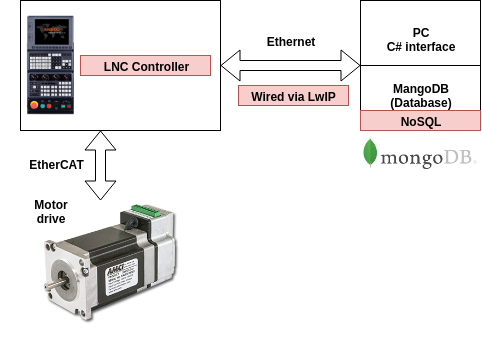
\includegraphics[width=0.7\textwidth]{Untitled.png}
      \end{center}
      \caption{Framwork of experiment.}
      \label{fig:}
    \end{small}
  \end{figure}
  
\end{frame}

\subsection{Primary Scenario}
\begin{frame}{Primary Scenario}{Outline of experiment environment}
  \begin{itemize}
    \item Setting up GUI for controller in C\# (provided by LNC Tech. )
    \item Connecting to controller via wired Ethernet.
    \item Uploading G-code for controller in C\# via File Transfer Protocol.
    \item Starting up motor drive by running uploaded G-code.
    \item Receiving encoder data and sending to server (.py) via socket.
    \item Listening to any client to be connected.
    \item Creating MongoClient, connecting to server and receiving data simutaneously.
    \item  Storing data into database and collection.
  \end{itemize}
\end{frame}

\subsection{Hardware}
\subsubsection{{LNC controller}}
\begin{frame}{Hardware}{LNC controller}
  \begin{columns}
    \begin{column}{0.48\textwidth}
      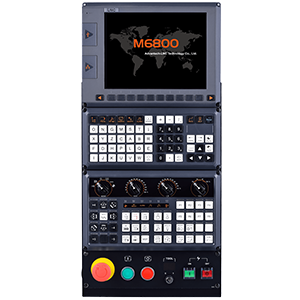
\includegraphics[width=\linewidth]{M6800-30020180627160202.png}
    \end{column}
    \begin{column}{0.7\textwidth}
      \small
      \begin{itemize}
        \item 10.4”TFT LCD.
        \item Control 9+6 axis.
        \item Support Mll/RTEX/ EtherCAT communication protocol.
        \item High-speed, high- precision and wiring saving.
        \item Provides interpolations to satisfy the requirements of high level of turn-milling.
        \item Various intelligent functions.
        \item Particle-button and support USB drive. \\\
      \end{itemize}
    \end{column}
\end{columns}
\tiny{Source: \url{https://www.lnc.com.tw/en-us/products/651310d3-07e8-4065-96e2-e9cee323a966/t6800d-m(vertical_pbo)/mod_4b83b157-94cd-45ad-a36e-0a85483f4009}}
\end{frame}

\subsection{Software}
\subsubsection{Socket}
\begin{frame}
  A mechanism for allowing communication between processes where running on same/different computers connected on a network.
  \medskip
\begin{columns}
  \begin{column}{0.55\textwidth}
    
\includegraphics[width=\linewidth]{socket.jpg}
  \end{column}
  \begin{column}{0.5\textwidth}
    \small
    
Widely used applications:
\begin{itemize}
  \item Instant messaging and chat.
  \item Real-time analytics by pushing data to clients that get represented as real-time counters, charts or log.
  \item Documentation collaboration. \\
\end{itemize}
  \end{column}
\end{columns}
\end{frame}

\subsubsection{MongoDB}
\begin{frame}{Software}{MongoDB}
  \begin{columns}
    \begin{column}{0.4\textwidth}
      
\includegraphics[width=\linewidth]{mongodb_logo1-76twgcu2dm.png}
    \end{column}
    \begin{column}{0.7\textwidth}
      \begin{itemize}
        \item Easy to install and set up.
        \item A BSON (a JSON-like format) to store data.
        \item Easy to map the document objects to application code.
        \item Highly scalable and available, and includes support for out-of-the-box replication.
        \item Support MapReduce operations for condensing a large volume of data into useful aggregated results.
        \item Free and open source.\\\
      \end{itemize}
    \end{column}
\end{columns}

\tiny{Source: \url{https://www.sitepoint.com/an-introduction-to-mongodb/}}
\end{frame}


\begin{frame}{Software}{MongoDB - NoSQL}
\begin{itemize}
  \item Flexible data models (Schema Free)
    \begin{itemize}
      \item NoSQL databases more relaxed in structure of data
    \end{itemize}
    \item Clusters of cheap commodity servers to manage the data and transaction volumes
    \item NoSQL are still implementing their basic feature set
\end{itemize}

Why MongoDB?
\begin{itemize}
  \item Simple queries
  \item Functionality provided applicable to most web applications
  \item Easy and fast integration of data
  \item Not well suited for heavy and complex transactions systems
\end{itemize}
\end{frame}

% ----- Basic ------
\section{Basic Scenario}
\subsection{Ethernet Connection}
\begin{frame}{Ethernet Connection}
TCPIP connection between LNC controller to PC.
\begin{figure}
  \centering
  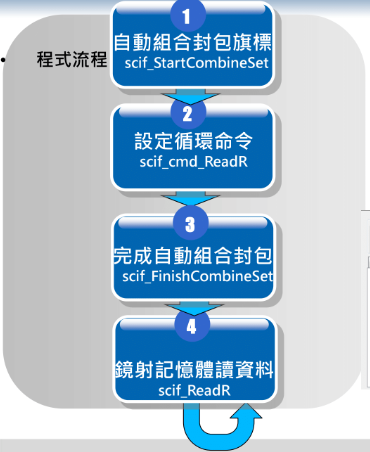
\includegraphics[scale=0.3]{controller.png}
  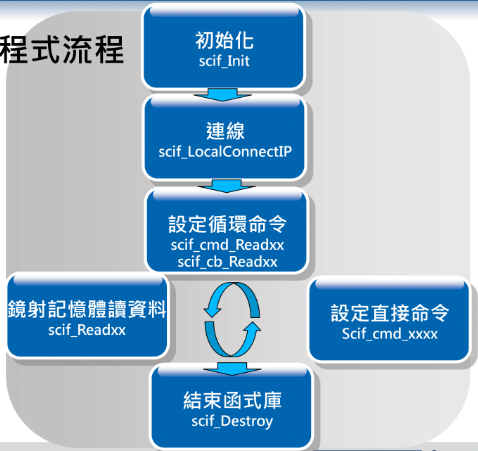
\includegraphics[scale=0.3]{controller2.png}
\end{figure}
\end{frame}
\begin{frame}{Ethernet Connection}
  TCPIP connection between LNC controller to PC.
  \begin{figure}
    \centering
    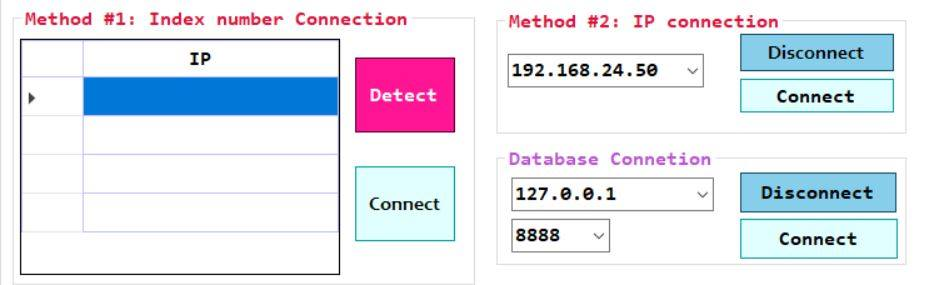
\includegraphics[scale=0.35]{ui3.jpg}
  \end{figure}
  \end{frame}

\subsection{Data Extraction}
\begin{frame}{Data Extraction}
\begin{itemize}
  \item Extract data (eg. coordinates, loading, error) stored in R values.
  \item Get polling of the mirror memory for important R values.
\end{itemize}
\begin{figure}
  \centering
  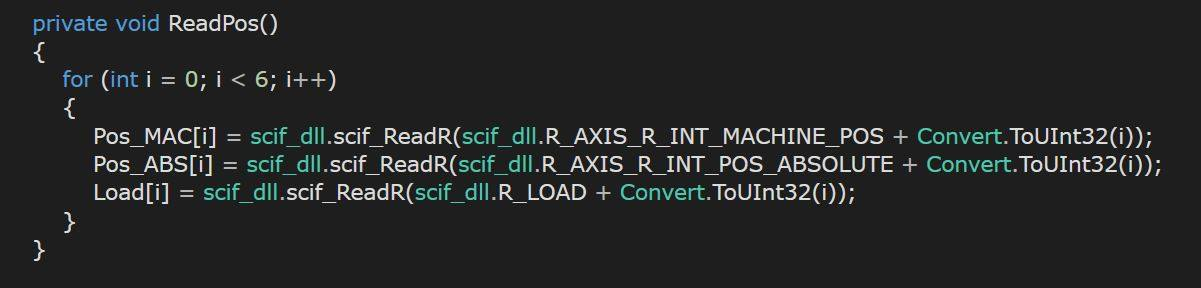
\includegraphics[scale=0.22]{data.jpg}
  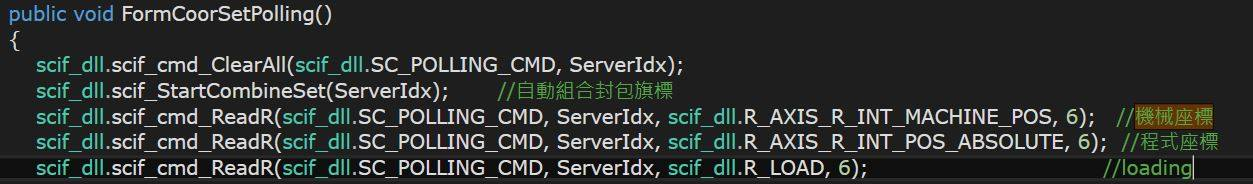
\includegraphics[scale=0.25]{data2.jpg}
\end{figure}
\end{frame}

\begin{frame}{Data Extraction}
  \begin{itemize}
    \item Extract data (eg. coordinates, loading, error) stored in R values.
    \item Get polling of the mirror memory for important R values.
  \end{itemize}
  \begin{figure}
    \centering
    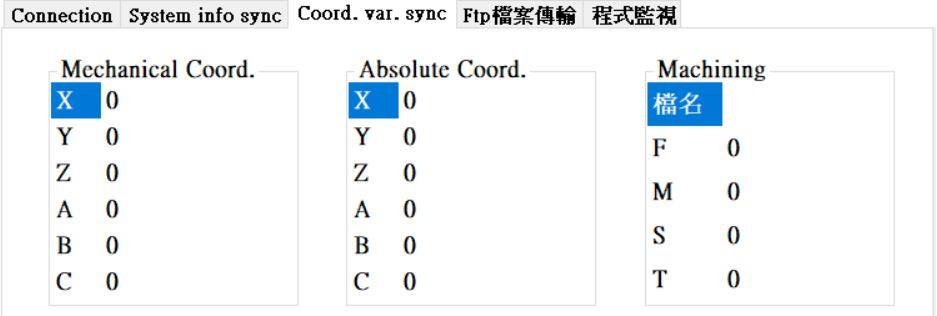
\includegraphics[scale=0.3]{ui2.jpg}
  \end{figure}
  
  \end{frame}


\subsection{Controller}
\begin{frame}{Controller}
  \begin{itemize}
    \item Using G-code to control the hardware
    \item Using Ftp file transmission to upload G-code 
  \end{itemize}
  \begin{figure}
    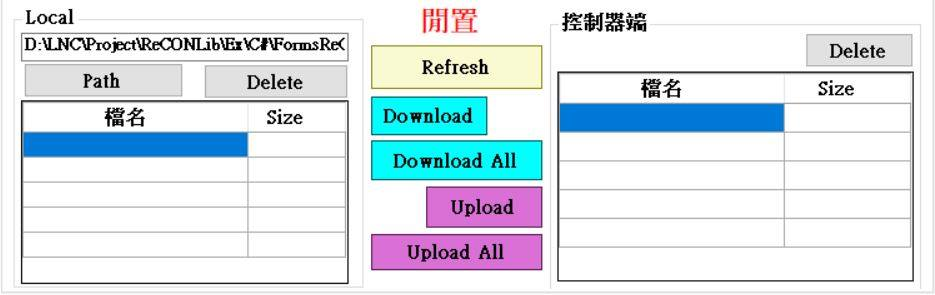
\includegraphics[scale=0.3]{ui.jpg}
  \end{figure}
\end{frame}

\subsection{Machining Process}
\begin{frame}{Machining Process}
  \begin{itemize}
    \item Similar to typical factory application.
    \item G-code allows users to select machining process.
    \item Two R Values for G-code
    \begin{itemize}
      \item ${\Phi R290100}$: Return to \textbf{0} when machining ends, set to \textbf{1} to start working
      \item ${\Phi R290101}$: Set \textbf{0} to go straight path to desired points; \textbf{1} to go curve path; \textbf{2} to stop machining
    \end{itemize} 
  \end{itemize}
  \begin{figure}
    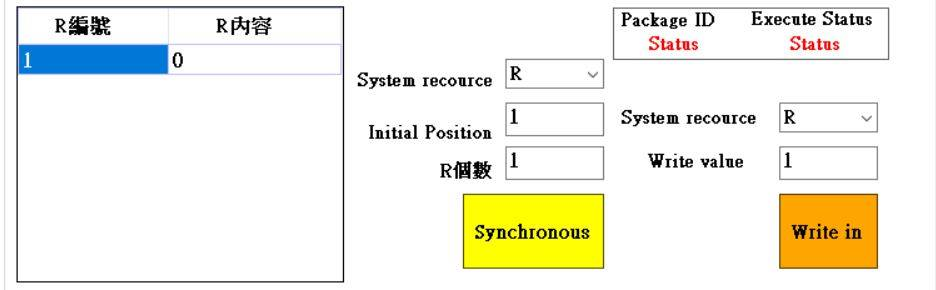
\includegraphics[scale=0.3]{ui4.jpg}
  \end{figure}
\end{frame}

\subsection{Data Transmission}
\begin{frame}{Data Transmission}
  \begin{itemize}
    \item LNC controller API function to Read R register value from Memory.
    \item \textbf{Socket} client(TCP) is created in same C\# program.
    \item Socket client connects to local host (127.0.0.1).
    \item Waiting for server's acceptance/response.
    \item Sending Position and Payload data to socket server every second counts.
  \end{itemize}
\end{frame}

\begin{frame}{Data Transmission}
  \begin{itemize}
    \item Create a python socket server and \textbf{listen} to any connection.
    \item Socket server \textbf{connect}s to local host (127.0.0.1).
    \item Receive (\textbf{recv}) data from client.
    \item \textbf{PyMongoClient} gets data from server also on local host.
    \item Database is created simutaneously.
  \end{itemize}
\end{frame}


\subsection{Primary Scenario Demo}
\begin{frame}{Demo}{Primary Scenario Demo}
  \centering
  \Huge{VIDEO}
\includegraphics[scale=0.025]{228-2283562_png-file-video-icon-vector-png.png}
\end{frame}

%----- Application -------
\section{Application Scenario}

\begin{frame}{Application idea}
Initially, we use R value of \textbf{Payload} as our main focus of optimization control. Therefore, the acceleration/deceleration of escalators reminds us of one of the key of the motion is depending on the magnitude of payload it endures.

As to realize this scenario, we've extended the basic scenario futhermore.
\end{frame}


\begin{frame}{Application Scenario}
  \begin{itemize}
    \item Setting up GUI for controller in C\# (provided by LNC Tech. )
    \item Connecting to controller via wired Ethernet.
    \item Uploading G-code for controller in C\# via File Transfer Protocol.
    \begin{itemize}
      \item \textcolor{red}{G-code reads loading R values and controls rotating speed.}
    \end{itemize}
    \item Starting up motor drive by running uploaded G-code.
    \item Receiving encoder (\textcolor{red}{\& payload}) data and sending to server (.py) via socket.
    \item Listening to any client to be connected.
    \item Creating MongoClient, connecting to server and receiving data simutaneously.
    \begin{itemize}
      \item \textcolor{red}{Dynamically updating plot in matplotlib.}
    \end{itemize}
    \item  Storing data into database and collection.
    \begin{itemize}
      \item \textcolor{red}{Find data from collection w/ or w/o query.}     
    \end{itemize}
  \end{itemize}
\end{frame}

\subsection{G-code Payload R values}
\begin{frame}{G-code Payload R values}
  G-code simulation.
    \begin{figure}
      \centering
      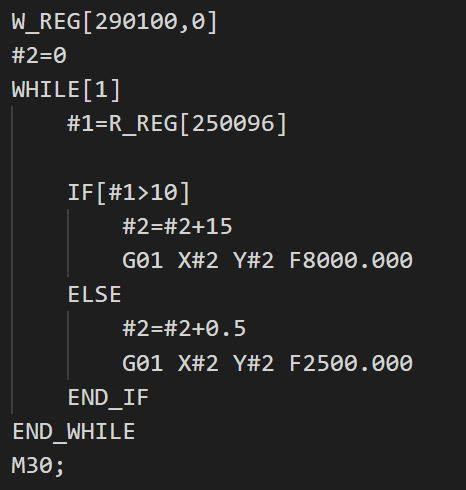
\includegraphics[scale=0.22]{g1.jpg}
      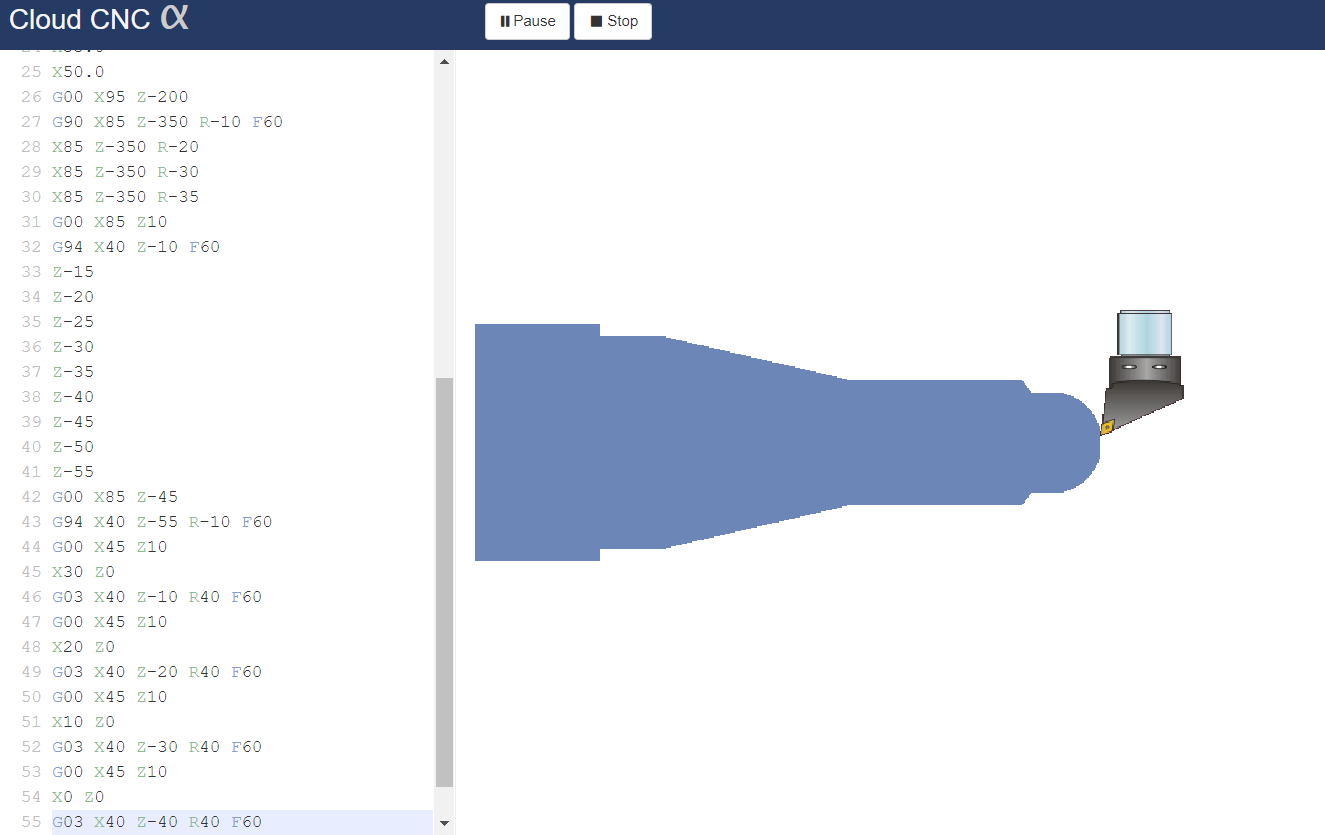
\includegraphics[scale=0.15]{actual.png}
    \end{figure}
  \end{frame}

\subsection{Dynamically Updating Plot}
\begin{frame}{Dynamically Updating Plot}
  Use \textbf{Matplotlib}, update figure and axis range once receiving data from database dynamically.
\end{frame}

\subsection{Find data}
\begin{frame}{Find Data}
  From another point of view, once the database is built, other clients can access to the database and look for data. For our case, we hope that user can find data by giving some information of time, and investigate the process situation during that time interval.
  \begin{figure}
    \centering
    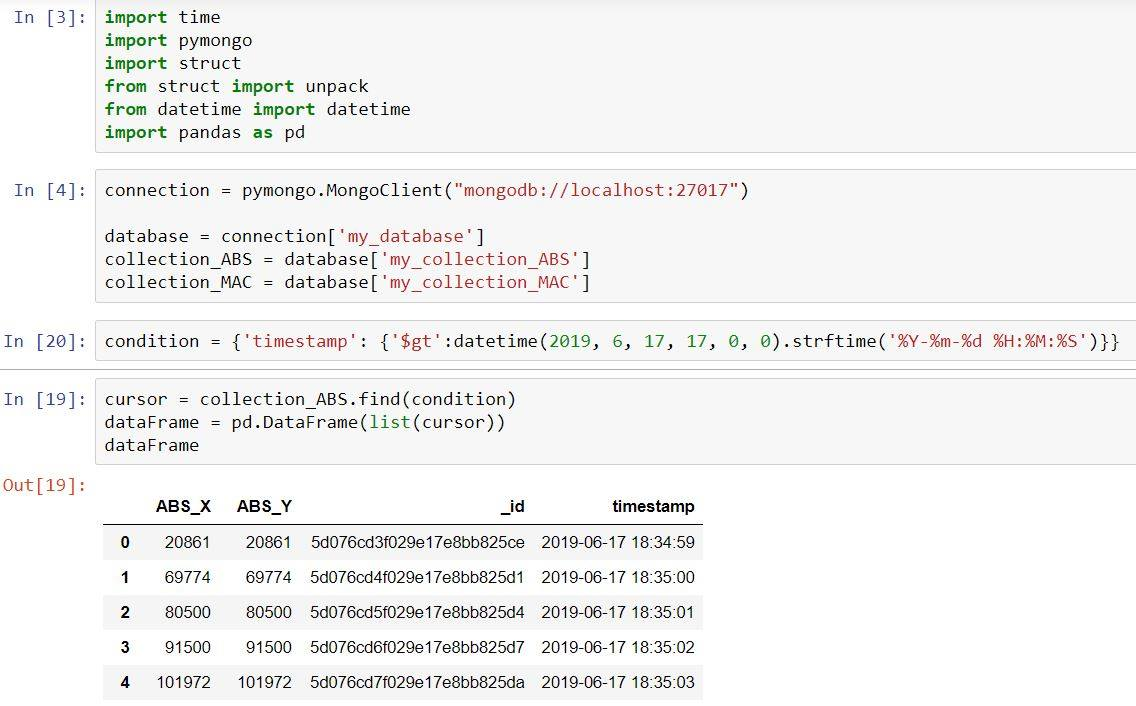
\includegraphics[scale=0.2]{query2.jpg}
  \end{figure}
\end{frame}

\begin{frame}{Find Data}
  \begin{figure}
    \centering
    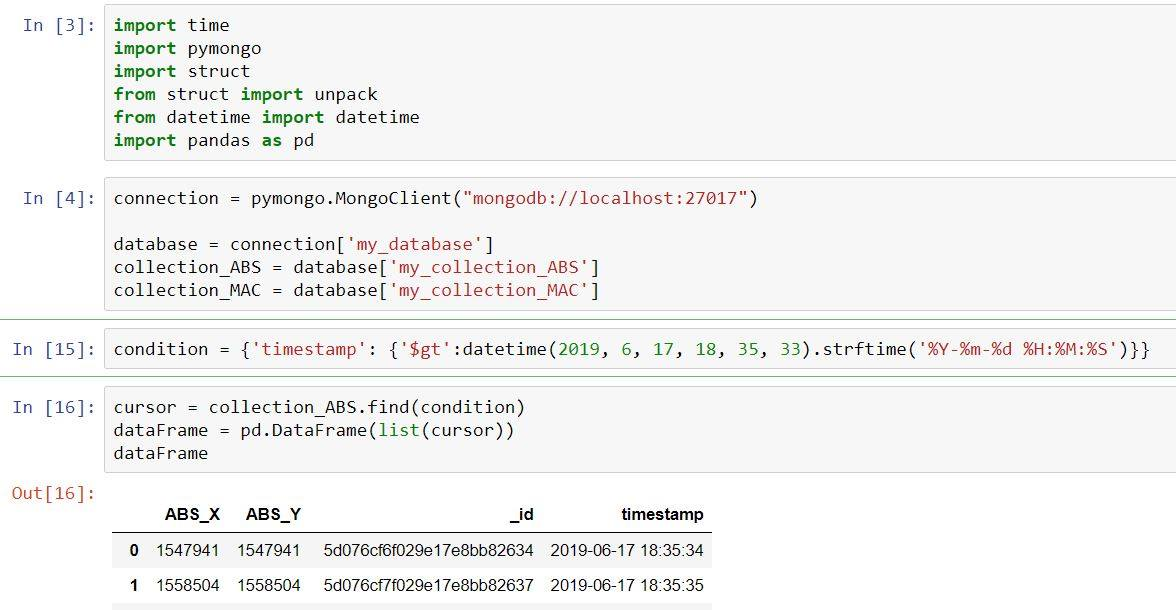
\includegraphics[scale=0.28]{query1.jpg}
  \end{figure}
\end{frame}


%------- Demo --------
\subsection{Application Scenario Demo}
\begin{frame}{Demo}{Application Scenario Demo}
  \centering
  \Huge{VIDEO}
  
\includegraphics[scale=0.025]{228-2283562_png-file-video-icon-vector-png.png}
\end{frame}


\section{Conclusion}
\begin{frame}{Discussions}
  \begin{itemize}
    \item We use python for database operation and C\# for Controller data synchronization. How to implement Inter Program Communication(IPC)?
    \begin{itemize}
      \item By Socket TCP, we send dataFrame from C\# interface to python server and bind local Host as IP address. 
    \end{itemize}
    \item Simulating the process\footnote{\tiny{\url{https://cnc-lathe-simulator.appspot.com/}}} can help users more easily monitor the entire machining process.
    \item Socket sends data stream in Bytes array. Thus, we take advantages of Concept of Union (The same memory address) and transform \textbf{Int} to \textbf{Bytes} array (1 Int = 4 Bytes in C\#). While  receiver decodes Bytes array back into Int.
  \end{itemize}
\end{frame}

\begin{frame}{Conclusion}
  Through C\# GUI to give commands to controller, and store data into the database at the same time is achievable. Data visualization and its noSQL structure can better improve data storage and management. Those applications can greatly optimize control in different scenarios.
\end{frame}

\begin{frame}
  \centering
  \LARGE
  Thank you! Any Question?
\end{frame}
\end{document} 


